\section{General Structure}

Our honeypot system is composed of a number of websites (500 in our experiments), each containing the installation of seven among the most common - and notoriously vulnerable - content management systems, and a static web site linked to 17 pre-installed web shells among the most common ones that can be found on the Internet, like c99 and priv57r.

A Generic overview of a website can be seen in figure~\ref{fig:websiteView}

\begin{figure}[tbh]
\centerline{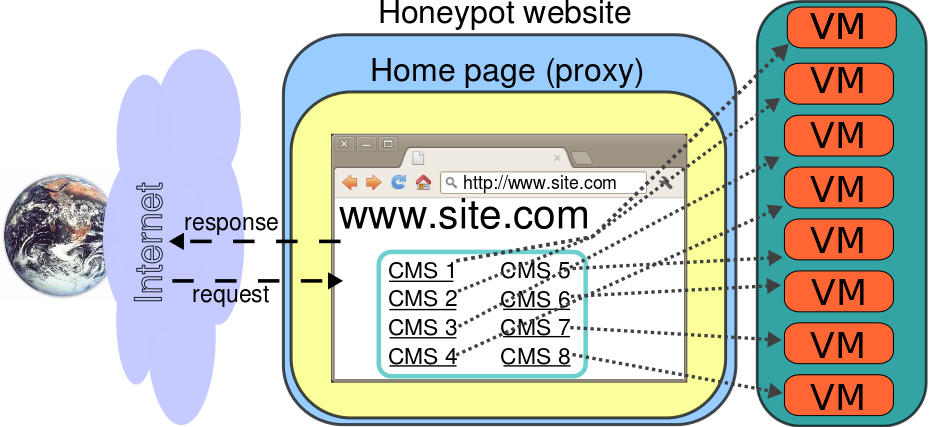
\includegraphics[width=0.9\textwidth]{Images/websiteOverview.png}}
\caption{Overview of a website.\label{fig:websiteView}}
\end{figure}

As can be seen, the system is composed by two main parts: A VMWare server, located in our facilities, hosting our web applications, and a total of 500 replicated web proxies hosted by TrendMicro distributed over eight different locations across the world, connecting the servers to the Internet. Any request reaching one of the web proxies is forwarded to our server, and the suitable response is sent back to the proxy and from there to the final user.

To make our honeypots reachable from web users, we purchased 100 bulk domain names on GoDaddy.com with privacy protection. The domains were equally distributed among the .com, .org, and .net TLDs, and assigned evenly among the locations.
On each of the eight locations, we configured four additional subdomains for every domain, obtaining five distinct websites (e.g, on domain site.com we have www.site.com, sub1.site.com, sub2.site.com, sub3.site.com and sub4.site.com). A schema of this structure is shown in fugure~\ref{fig:genSchema}

\begin{figure}[tbh]
\centerline{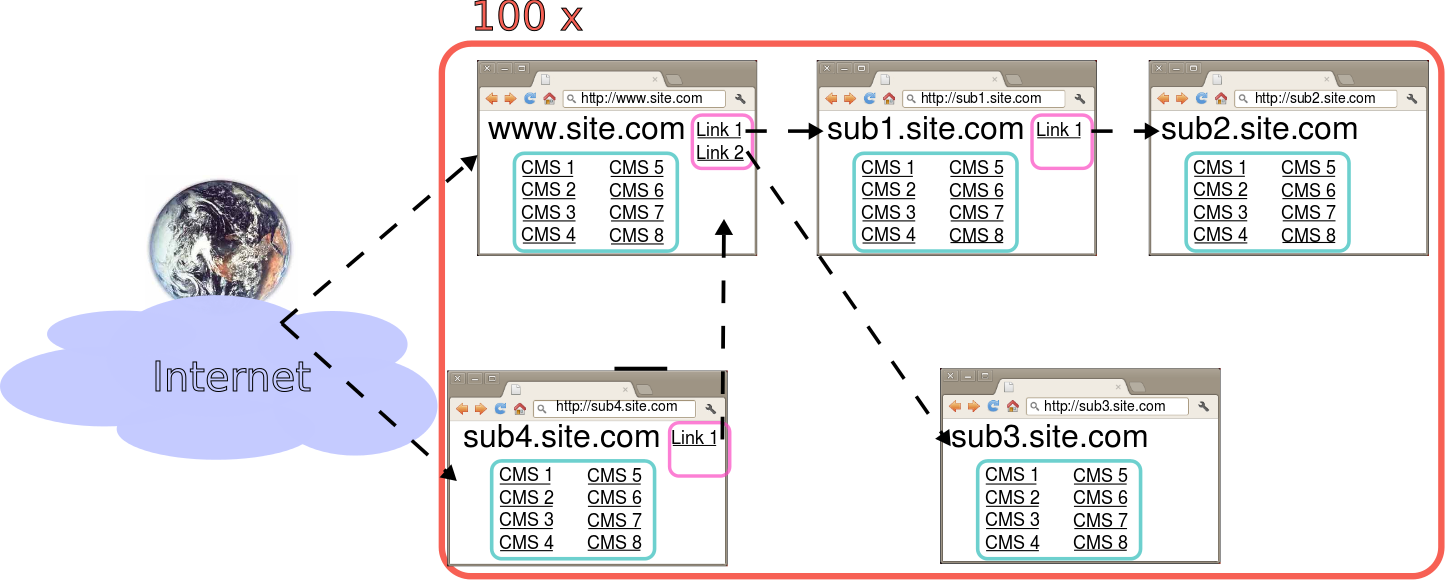
\includegraphics[width=0.9\textwidth]{Images/GeneralSchema.png}}
\caption{General schema of the honeypot platform.\label{fig:genSchema}}
\end{figure}

Finally, we advertised the 500 domains on the home page of the authors and on the research group's website by means of transparent links. This approach, initially proposed by M\"uter et al. \cite{hihat}, consist in adding on high-reputation web pages links not visible by the user to other pages, so that the position of these latter ones in the Google index will increase.

In order to manage such a high-number of different machines in a comfortable way we used a modified version of \emph{ftp-deploy} script to upload, in batch, every file we needed to each of the 500 websites in our possession. This greatly simplified the deployment and the update/upgrade of the system, and solved one of the main issues developers need to solve during the deployment of replicated content over different providers. Even if the hosting services can always be traced back to Trend MicroSystems, in fact, each of them has its own directory structure and specific web interface, discouraging the usage of ssh and other advanced management options in order to deploy contents. Thus the only way to easily perform this action was to use FTP protocol, the only one supported by every provider.

Looking more closer to figure~\ref{fig:genSchema}, It can be noticed as the linking structure is not the same for every subdomain. Indeed, each subdomain links to at most 2 different subdomains under its same domain. The aim of this particular structure of the linking graph is to detect possible malicious traffic from systems that automatically follow links and perform automated attacks or scans.

\section{The Web Applications}
We deployed a total of eight web servers, using seven web applications and one static web site linked to 17 pre-installed webshells. Every web application is based on an openSource Content Management System among the most used across the Internet, each one based on php version 5 and using (if needed) MySQL version 5 as RDBMS. For each CMS, we chose a version with a high number of reported vulnerabilities, or at least with a critical one that would allow the attacker to take full control of the application. We also limited our choice to versions no more than 5 years old in order to ensure our websites are still of interest to attackers.
Our choice was guided by the belief that attackers are always looking for low-hanging fruits. On the other hand, our honeypots will probably miss sophisticated and unconventional attacks, mostly targeted to high profile organizations or well known websites. However, these attacks are not easy to study with simple honeypot infrastructures and are therefore outside the scope of our study.

\textcolor{blue}{NOTE: Depending on the output, maybe it's better to create different subsubsection for each web application, or leave it as it is right now. NO I LIKE WITH DESCRIPTION. \\
I like the idea of putting a reference with a link to the exploit at the bottom, from exploit-db.com. However i don't like it to have such a englight over the page, maybe removing url? leaving it like a normal text?}

\begin{description}
\item[phpMyAdmin: ] phpMyAdmin \cite{phpMyAdmin} is an openSource tool written in PHP for the administration of a MySQL database over the WWW. The version installed is the 3.0.1.1 disguised as version 2.6.4-rc1. Both these versions present a critical PHP code injection vulnerability in the \"/scripts/setup.php\", a page needed during the installation process of the CMS which should be manually uninstalled at the end of it, allowing an attacker to inject a payload that can execute arbitrary PHP commands. Even if both versions are vulnerable to this exploit, a research over various underground forums showed as the one for the version 2.6.4-rc1 is far more well-known with respect to the 3.0.1.1 one (even if they are identical), thus we disguised our version to the one more suitable for attackers (the 2.6.4-rc1 is no more available for downloads on phpMyAdmin website).
Reference:
\begin{itemize}
\item
\url{http://www.exploit-db.com/exploits/8921/}
\end{itemize}

\item[osCommerce: ] osCommerce \cite{osCommerce} is one of the most used openSource e-commerce and online store-management frameworks. Our specific version is the 2.2, which contains several critical vulnerabilities, from arbitrary file upload to modification of admin user and password by anonymous user.
Reference:
\begin{itemize}
\item
\url{http://www.exploit-db.com/exploits/16899/}
\item
\url{http://www.exploit-db.com/exploits/9566/}
\item
\url{http://www.exploit-db.com/exploits/10707/}
\item
\url{http://www.exploit-db.com/exploits/12801/}
\end{itemize}

\item[Joomla!: ] Joomla! \cite{joomla} is an openSource general-purpose framework. The version we used is the 1.5, with the addition of two plugins, tinybrowser 1.0 (a plugin for listing directories and file management) and com\_graphics 1.0.16 (magnify ability to the page). This web application suffers from several vulnerabilities both server and client-side, admin password reset, remote file inclusion, local file inclusion and multiple XSS (Cross-Site scripting) cause by bad input filtering.
Reference:
\begin{itemize}
\item
\url{http://www.exploit-db.com/exploits/6234/}
\item
\url{http://www.exploit-db.com/exploits/16091/}
\item
\url{http://www.exploit-db.com/exploits/12430/}
\item
\url{http://www.exploit-db.com/exploits/9926/}
\end{itemize}

\item[Wordpress: ] Wordpress \cite{wordpress} is a popular CMS aimed to the easy creation of a blog. Our version is the 2.8, with one plugin installed, kino version 1.1, a calendar/event manager, and a theme, amphion-lite. Both the plugin and the theme rely on the file timthumb.php, vulnerable from Remote File Inclusion vulnerability. This is a website which allowed to post comments, therefore we needed to take care of removing offensive/illegal content from the posts. Anyone can register to the website, and the default user role is Contributor, allowing creation of posts with links but not file uploads. Posts are sanitized from links and then become viewable to guests. For this particular machine we had to authorize sending emails because of the registration procedure, but we stop email scams by the analysis of the content of each single mail the server is willing to send.

Reference:
\begin{itemize}
\item
\url{http://www.exploit-db.com/exploits/17872/}
\end{itemize}

\item[SMF: ] SMF (acronym of Simple Machines Forum \cite{smf}) is an openSource software for developing a forum web application, where users can open threads and post comments. Our specific version is the 1.1.3. As in the case of the Wordpress machine, we applied the same approach for managing registration via mail and for checking posts on the forum. This application suffers from several vulnerabilities, the most important ones are a remote PHP code execution vulnerability, a stored XSS and an information-disclosure vulnerability.
Reference:
\begin{itemize}
\item
\url{http://www.exploit-db.com/exploits/10274/}
\end{itemize}

\item[Static website: ] We also created a static website composed only by HTML pages with a hidden directory containing 17 different web-shells. These web-shells have been taken from underground forums and past experiments, and are fully equipped in order to perform any operation an attacker would like to perform, from shell commands execution to full database dump. They are indexed by search engine and can therefore easily be found by an appropriate dork.

\item[Wordpress: ] Because of the dominant position of Wordpress CMS on the market, we deployed another web application based on this system. This specific machine run an updated version of Wordpress (3.4) with two plugins, wpstorecart and nextgengallery. Both these plugins suffer from Arbitrary File Upload vulnerability.

\begin{itemize}
\item
\url{http://www.exploit-db.com/exploits/19023/}
\item
\url{http://1337day.com/exploit/description/20352}
\end{itemize}

\item[Drupal: ] Drupal \cite{drupal} is the third most common CMS present on the web, after Wordpress and Joomla!. We installed version 7 of this application with IMCE plugin (Image manager). This machine does not present a standard vulnerability, but rather a mis-configuration: IMCE allows for remotely upload files inside a specific directory, and its access should be denied for every user but the administrator. In this case this page is usable by every user, and it's also indexed by search engines.
\end{description}

Table~\ref{tab:webapps} shows a summary of the web applications used and its vulnerabilities.

\begin{table}[tbh] % per piazzare la tabella t:top b:bottom h:here in ordine di preferenza; h è sconsigliato
\begin{center}
\begin{tabularx}{\textwidth}{|c|X|X|X|X|}
\hline
\textit{VM \#} & \textit{CMS, version} & \textit{Plugins} & \textit{Description} & \textit{Vulnerabilities} \\
\hline
1 & phpMyAdmin, 3.0.1.1 & - & MySQL database manager & PHP code injection \\
2 & osCommerce, 2.2 & - & Online shop & 2 remote file upload, arbitrary admin password modification \\
3 & Joomla, 1.5.0 & com\_graphics, tinymce & Generic / multipurpose portal & XSS, arbitrary admin password modification, remote file upload, local file inclusion \\
4 & Wordpress, 2.8 & kino, amphion lite theme & Blog (non moderated comments) & Remote file include, admin password reset \\
5 & Simple Machines Forum (SMF), 1.1.3 & - & Forum (non moderated posts) & HTML injection in posts, stored XSS, blind SQL injection, local file include \\
6 & PHP web shells, static site & - & Static site and 17 PHP shells (reachable through hidden links) & PHP shells allow to run any kind of commands on the host \\
7 & Wordpress, 3.4 & wpstorecart, nextgengallery & Blog & Arbitrary File Upload \\
8 & Drupal, 7.0 & IMCE & Generic / multipurpose portal & Remote File Upload \\
\hline
\end{tabularx}
\caption{Summary of the web applications deployed on the system.\label{tab:webapps}}
\end{center}
\end{table}

\section{The Web Proxy}

The Web Proxy is in charge of receiving the various requests from the Internet, creating a unique channel for the communication between the user and the vulnerable webserver and propagating the requests to the gateway.
All web applications are hosted in our facilities, in eight isolated virtual machines running on a VMWare server. On the proxy hosting side we installed only an ad-hoc proxy tool (HoneyProxy) in charge of forwarding all the received traffic to the right virtual machine on our server.

We crafted a custom install of the Apache webserver using modified .htaccess file, ModRewrite module, cURL module and php.ini configuration files, in order to be able to transparently forward the user requests to the appropriate URL on the corresponding virtual machine. Any attempt to read a non-existing resource, or to access the proxy page itself would result in a usual 404 error page shown to the user. Not taking into account possible timing attacks or intrusions on the proxy hosting servers, there is no way for a visitor to understand that he is speaking to a proxy.

The HoneyProxy system installed on every website is composed of an index file, the PHP proxy script itself and a configuration file. The index file is the home page of the website, and it links to the vulnerable web applications and to other honeypot websites, based on the contents of the configuration file. The proxy uses sessions in order to serve the appropriate page to each user, and it also scans each response received from the web application before forwarding it in order to substitute each domain with the one initially requested by the user.

Furthermore, The PHP proxy adds two custom headers to each request it receives from a visitor:

\begin{description}
\item[X-Forwarded-For: ] this standard header, which is used in general by proxies, is set to the real IP address of the client. In case the client arrives with this header already set, the final X-Forwarded-For will list all the previous IPs seen, keeping thus track of all the proxies traversed by the client. This is necessary in case the user passes through another proxy before reaching ours.

\item[X-Server-Path: ] this custom header is set by our PHP proxy in order to make it possible, for us, to understand the domain of provenance of the request when analyzing the request logs on the virtual machines. An example of such an entry is: X-Server-Path: http://sub1.site.com/. This entry will be used to substitute all references to other resources inside each page before sending it to the user.
\end{description}

These two headers are transmitted only between the hosting webserver and the honeypot VM's webserver, and thus they are not visible to the users of the HoneyProxy.

\section {The Gateway}

The Gateway is in charge of sorting the requests coming from the proxy to the appropriate webserver. This is the only communication channel between the vulnerable web applications and the outside world, and it's therefore a critical point for the infrastructure.
This machine runs a very basic Debian version, with a complex routing table and a complete set of firewall rules based on iptables. We provided this machine with two connections to the Internet: the main one, where the requests to/from the honeypots are going through, which is based on a point-to-point VPN connection to the proxy, and a secondary line which is directly connected to the outside world via a DSL connection.

The general approach on which the gateway relies in order to solve connections is the following:

\begin{description}
\item[Requests coming from the proxy: ] this requests are coming from the point-to-point VPN connection. The proxy already changed the request in such a way that the destination port will be specific to the web application the request is directed to. The proxy simply receives the request, changes the destination port to the usual 80 and sends the request to the appropriate web application.

\item[Request coming from a web application: ] when the gateway receives a request coming from one of the webservers, it tries to understand its nature. If it's a HTTP response, it will forward it to the Proxy as a normal gateway, if it's something else (a beginning SSH connection, a raw IP packet or something else) it immediately drop the request and dump it on a log which will be analyzed daily. There are two exceptions to this behavior, explained in the following points.

\item[DNS requests coming from a web application: ] DNS requests represent an exception to the normal behavior. This kind of requests are forwarded to the Internet by the gateway using the secondary line. This behavior allows for the request to be solved without passing through the web proxy. The Proxy, in fact, is not hosted in our facilities and some malicious DNS could be blocked by the hosting provider. In this way we are sure that every DNS request is solved independently from the target of the request.

\item[HTTP requests coming from a web application: ] this represents the second class of exceptions to the normal behavior of the Gateway. In this case, in fact, we want to log the content of the HTTP request, which would be impossible if we instantaneously drop the first packet received. The natural sequence of actions performed during such an event is, in fact:
\begin{itemize}
\item an initial TCP SYN packet from the client to the server;
\item the server will answer with a TCP SYN/ACK packet;
\item the client will send a TCP ACK packet and the actual HTTP request;
\end{itemize}
Because we are interested in the last one of these packets, we used an extension of iptables called ``conntrack'' \cite{conntrack} which allows for tracking the entire connection and stop (and log) it when the first HTTP request is performed.
\end{description}

\section{The VMWare Server}

The VMWare server is the container of our web applications. Each web application is encapsulated in a different virtual machine hosted on this server. This allows for a fast recovery of any web application after a successful attack; this recovery is performed daily.
Our aim is to provide a properly safe environment for each web application, guaranteeing not only the undetectability of the presence of the virtual machine (the attacker should think to face a normal web server, not a honeypot), but also disallowing any action that can harm any other system outside our honeypots (e.g., in case a DoS script toward another server is run from one of our machines). Furthermore, we needed to prevent our honeypots to host any malicious or illegal content that could be dangerous for any client visiting the webpage.
We studied every possible threat that could endanger our honeypot system, and we tackle each of these problems separately.

\subsubsection{Gaining high privileges on the machine}

 We tackled this problem by using a double protection. First, all our web application run in a completely updated VMWare virtual machine, which is considered pretty safe (the last known escaping vulnerability is CVE-2008-0923 by Core Security Technologies \cite{vmescape}). On this virtual machine there is a further protection, as the vulnerable processes run inside an LXC container. This technology provides an operating system-level virtualization that has its own process and network space. Basically we are building multiple cages one inside the other in order to guarantee that no possible attacks can reach our real machine. Inside this container, we installed only basic linux tools (in particular, they are python, perl, wget, cURL, build-essentials) and the two services needed for the web application to work, apache and mysql. This approach does not guarantee absolute protection, but in order to reach the real servers an attacker should need at least one 0-day exploit for apache, one for LXC and one for VMWare, which is obviously a very remote possibility.

\subsubsection{Using the honeypot machine as a stepping stone to launch attacks or email campaigns}

 This is probably the most important threat a high-interaction honeypot system should face when it's been deployed on the Internet. We wanted to trick the attacker into feeling that his system works, but without actually doing any real action instructed by the malicious user. Outgoing connections starting from our machine are blocked by a specific set of \emph{iptables} rules. Furthermore, the connMark plugin for iptables allowed us to fool the attacker into thinking the machine can actually connect to the outside. As mentioned before, we allow the first and second packet in the TCP three-way handshake , but we disallow the final third packet. This provokes most of the tools used to establish a TCP connection (wget, cURL, netCat) to display a \emph{``Connection Established''} message, tricking the attacker into thinking that the outside server is suffering from connectivity problems. Furthermore, this allowed us to collect not only data relative to the IP of the target server, but also specific queries, as specific web addresses of malicious scripts. We also set a limit to the maximum number of connections that can be established in this way between one of our servers and an outside world in order to prevent our servers to be used as a SYN flood Denial Of Service attack starting platform.

\subsubsection{Hosting and distributing illegal content(e.g., phishing pages)}

 It is virtually impossible to completely disable this threat if our web applications have remote file upload vulnerability. An attacker could always upload a phishing pack and then advertise the link to it using another server, fooling the victims into the malicious page. In any case, we mitigate this risk by limiting the directories where files can be uploaded and preventing any modification to existing files on the machine, so that attackers can't, for example, replace the index page of our web servers. As a precautionary measure, we also monitor every change happened in the LXC container file system and in the VM. If such a modification is detected, the system takes a snapshot of the VM. Each VM is restored to its original snapshot at regular intervals, preventing potentially harmful content from being delivered to victims or indexed by search engines.

\subsubsection{Illegal promotion of goods or services (e.g., spam links)}

 Some of our applications allowed for some degree of interaction with users from the Internet, like insert comments to blog entries or publish posts in case of the forum. These kind of applications are heavily targeted by spammers, and we wanted to be sure that links and posts published by malicious users would not reach regular users or be indexed by search engines. Luckily for us this activity is almost fully accomplished by automatic scripts, therefore we were able to directly modify the source code of the interested web application, commenting out each snippet of code responsible of showing any spam link or related content. In this way, attackers can still publish content (and we log every single post they make), but a manual check of the webpage would show blank message instead of the malicious' payloads.
